\chapter{Evaluation}
\label{chap:evaluation}
In this section, we evaluate the performance of LiteBot against a custom test suite. Our evaluation consists of two main tests designed to assess different aspects of the algorithm.\\
In the first test we examine how well our modified Kabsch-Umeyama algorithm handles varying levels of noise helping us understand its stability and robustness to perform well even in noisy environments.\\
The second test compares different keypoint matching algorithms by using them in a full run of the algorithm and measuring their performance under identical environmental conditions. Following this test we will determine the best algorithm for use in our project, finalising the implementation design.

\section{Sensitivity to noise}
\label{sec:noise-test}
%evaluate how the kabsch algorithm performs with noise applied to ideal keypoints
In this test we want to understand how robust our modified Kabsch-Umeyama algorithm is to noise in the coordinates it receives. The hope is that small deviations to the coordinate inputs produce very small changes in the output translation and rotation matrix. If this is the case then the algorithm is robust to noise, and is more likely to produce good results when used in our system.\\

%TODO should really make a bigger suite, update number if we do
In order to conduct this test we create a test suite of 5 diverse objects and an accompanying demonstration for each one. We then manually mark an ideal set of keypoints in the demonstration image. These keypoints are recorded as a list of (x,y) pixel coordinate pairs. We also make sure to record the position and orientation of the object in the demonstration. We then place this same object in a different pose in the environment and save the live image from the robot in this case. Again making sure to note down the position and orientation of the object in this new scene. We then again manually mark the same keypoints but in this new image. \reftab{tab:test-suite} shows the transformation between the demonstration and live object pose. We also disclose how many keypoints were manually marked for each object. For further details about the specifics of the test suite, refer to \refapx{apx:test-suite}.\\

\begin{table}[h!t]
    \begin{adjustbox}{center}
    \renewcommand{\arraystretch}{1.2}
        \begin{tabular}{| >{\columncolor{lightgray!25}}c | c | c | c |}
            \hline
            \rowcolor{lightgray!25}
            Object & Translation applied & Rotation applied & Number of keypoints \\
            \hline
            Lego & [-0.1, 0.05, 0] & [0, 0, $\frac{\pi}{3}$] & 4\\
            \hline
            Mug & [0, 0.05, 0] & [0, 0, $\frac{\pi}{6}$] & 16\\
            \hline
            Ball & [-0.1, 0.07, 0] & [0, 0, 0] & 7\\
            \hline
            Jenga & [0.09, 0.15, 0] & [0, 0, $-\frac{\pi}{6}$] & 22\\
            \hline
            Domino & [0.05, 0.07, 0] & [0, 0, -$\frac{\pi}{4}$] & 10\\
            \hline
        \end{tabular}
    \end{adjustbox}
    \caption{The true transformation between demo and live objects in the test suite}
    \label{tab:test-suite}  
\end{table}

Now we can convert the manually marked keypoints in the demonstration and live image to world coordinates and pass them to our modified Kabsch-Umeyama algroithm. This should output the exact translation and rotation between the object from the demonstration to the live scene, within a small tolerance of floating point accuracy. The purpose of using human provided, ground truth keypoints is to control any additional noise in the test. If we used our keypoint matching algorithm then it would be unclear how much error came from our randomly added noise, or from mismatches in the keypoint algorithm. As such we gain clearer results by using our ground truth keypoints. With the method defined, we now add some noise to the ideal keypoints before passing them to the algorithm. We wish to compare how far the new output deviates from the true output when the noise is added. Since we add random noise, we conduct multiple runs and compute the average.

\subsection{Coordinate noise}
\label{subsec:coordinate-noise}
In this first set of tests the noise added is calculated as a random 3D unit vector multiplied by some random magnitude. When computing the random 3D unit vector, we take care to use an \speech{equal area projection of the sphere onto a cylinder} \cite{cylinder-proj}. This allows us to choose a point uniformly from the unit sphere, without experiencing a bunching of points at the poles \cite{uniform-3d-vector, random-vector}. This random noise is applied to the world coordinates after they have been computed from the ideal keypoints. This gives us a solid grasp as to just how much noise can be present before the algorithm produces unsatisfactory results.\\

\begin{figure}[h]
    \centering
    \begin{subfigure}[t]{0.49\textwidth}
        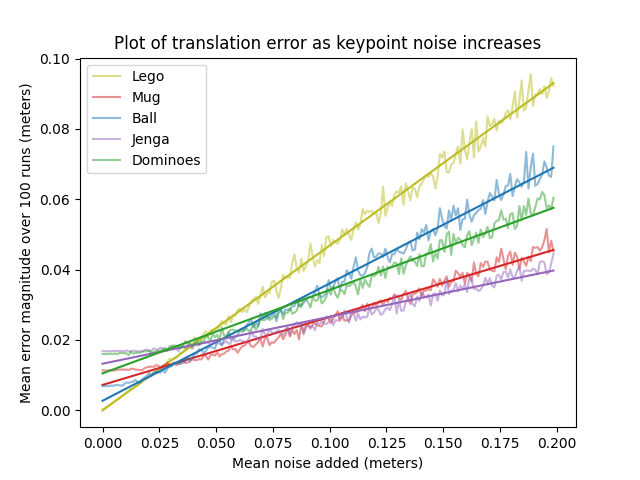
\includegraphics[width=\textwidth]{figures/fig_coordinate_noise-translation.png}
        \caption{Noise graph for translation error}
        \label{fig:noise-coord-translation}
    \end{subfigure}
    \hfill
    \begin{subfigure}[t]{0.49\textwidth}
        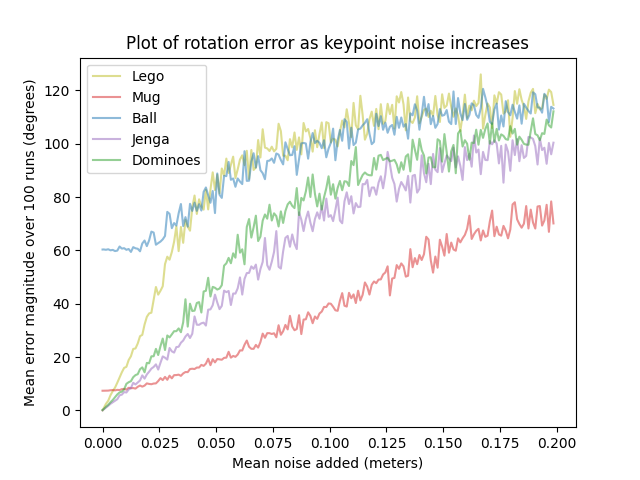
\includegraphics[width=\textwidth]{figures/fig_coordinate_noise-rotation.png}
        \caption{Noise graph for rotation error}
        \label{fig:noise-coord-rotation}
    \end{subfigure}
    \caption{Sensitivity analysis with added keypoint coordinate noise}
    \label{fig:noise-coord}
\end{figure}
In these tests noise was added within a range of 0.001 meters. The point plotted at horizontal coordinate $x$ was the result of sampling the noise magnitude from the half open interval $[x-0.0005,\: x+0.0005)$. This is with the exception of the data point at $x=0$. This point is the error when no noise was added, as though sampling the noise magnitude from $[0,0).$

\subsubsection{Translation error}
We see in \reffig{fig:noise-coord-translation} that the magnitude of the error between the true translation and computed translation appear to follow linear trend lines for all of the objects. A key observation is that the lines do not all intersect with the origin. This conveys that even with no added noise, the computed translation is still not the true translation. This systematic error remains constant across all results for the same object, only affecting the vertical intercept of the line, and not the gradient. This systematic error can be attributed to two main causes. Slight numerical precision errors will be present in the algorithm. These are somewhat exacerbated by converting our keypoints to world coordinates first. As a result keypoints, which are often very close to each other, have coordinates which differ only in low order decimal places. However, the much larger contribution to this systematic error is human error. The ground truth keypoint matching was performed by a human, and as a result is subject to large inaccuracies. It can be very difficult to identify the exact pixel which correspond between the demonstration and live image, especially when rotations and perspective distort straight edges.\\

For our test we are more concerned with how the error changes as a result of increasing the amount of noise the algorithm is subjected to. Therefore, we care more about the gradient of the trend lines than the true values. From this graph we can notice an interesting correlation. The gradient of each line is inversely proportional to the number of keypoints we marked. The Jenga block with the most keypoints is the most stable to additional noise, evident by possessing shallowest gradient. Meanwhile, the Lego piece with the fewest marked keypoints is the most sensitive. This relation holds for all intermediate objects with no outliers.\\

We also notice that even the worst performing object, the Lego piece, has a gradient less than 1. The line appears to have a gradient of approximately $\frac{1}{2}$, when ~20cm of noise is added, the error magnitude is ~10cm. This is promising because it is unlikely that the true noise experienced would be as high as 20cm. The graph shows that all objects were very stable up to 5cm of noise. This is a much more reasonable and still fairly generous estimate for how much noise the system will experience.\\

This result is quite promising for us, since the sensitivity appears to decrease as we mark more keypoints. We also note that the number of keypoints in this test are very low, due to requiring a human to manually place them. We will see in \refsec{sec:algos-test} that certain keypoint algorithms can identify on the order of thousands of keypoint matches. While this is dependent on the object used, it is promising as to the reliability of the system when automatic keypoint algorithms are used.

\subsubsection{Rotation Error}
\reffig{fig:noise-coord-rotation} shows how the rotation error increases as the amount of noise increases. The rotation error is computed as the geodesic distance between the rotations. Formally we consider the true rotation matrix $\hat{R}$ and the computed rotation matrix $R$ as representing orientations within 3D space. We then compute $E$, the error rotation matrix which rotates from $R$ to $\hat{R}$. $E$ represents how much more rotation we needed to do to get to the correct total rotation. $E$ represents a rotation by some angle $\theta$ about some axis. We consider $\theta$ to represent the size of this error, and is therefore our dependent variable. 
$$E = R^T \cdot \hat{R}, \longspace \theta = \frac{trace(E) - 1}{2}$$

Unfortunately, \reffig{fig:noise-coord-rotation} clearly shows that the algorithm is much more sensitive to noise when computing the rotation matrix. The trend lines in this graph do not appear to be linear for all objects. The error appears to increase more rapidly, before slowing down and reaching a plateau. The mug object appears to be most stable however, even this can reach quite large errors.\\

We again notice that the lines do not cross the origin due to systematic error. However, this time there is an outlier. The ball object has a rotation error of ~60 degrees with the human marked keypoints. This is not a small error due to inaccuracies in the keypoint placement, this is a fundamental issue with the Ball object. As shown in \refapx{apx:test-suite}, the keypoint placements on this object are not well placed to determine rotation. 6 of the 7 keypoints are placed around the perimeter of the ball. These mark the silhouette of the ball, which since it is a perfect sphere, would not change with a pure rotation. These keypoints are very useful for determining the translational offset, but they are no help in computing the rotation. This leaves a single keypoint placed in the middle of the object. The position of this keypoint, particularly its depth, is the only information the system has for computing how the object has rotated. Obviously this is insufficient, and leads to the very large error in \reffig{fig:noise-coord-rotation}. However, we will see in \refsec{sec:algos-test}, that even with many more keypoints, the system struggles to determine the rotation of the Ball object for the exact same reason. The majority of detected keypoints are on the edges of objects since this is when the image drastically transitions from the object to the background.\\

It is to be expected that rotation would be more sensitive to the noise than translation. Consider \reffig{fig:noise-difference} which shows a simplified view of this concept. We can see that for translation, the most unlucky we can get with the noise is for all of the noise vectors to align. If the noise vectors all had length n, then this would produce a translation error of n. This is why in \reffig{fig:noise-coord-translation}, the gradient of the trend lines were all less than 1. The absolute worst case is that the translation error would be equal to the noise magnitude. Since this is very unlikely and we compute an average, the trend lines are much more shallow than this worst case. However, for rotation, the worst case is that the noise vectors are all rotated copies of each other. We can clearly see by inspecting the figure, that this rotates the object by a much more noticeable amount, even when the same magnitude of noise is applied. This is why the rotation error is much more sensitive to the noise than the translation error.

\begin{figure}[h]
    \centering
    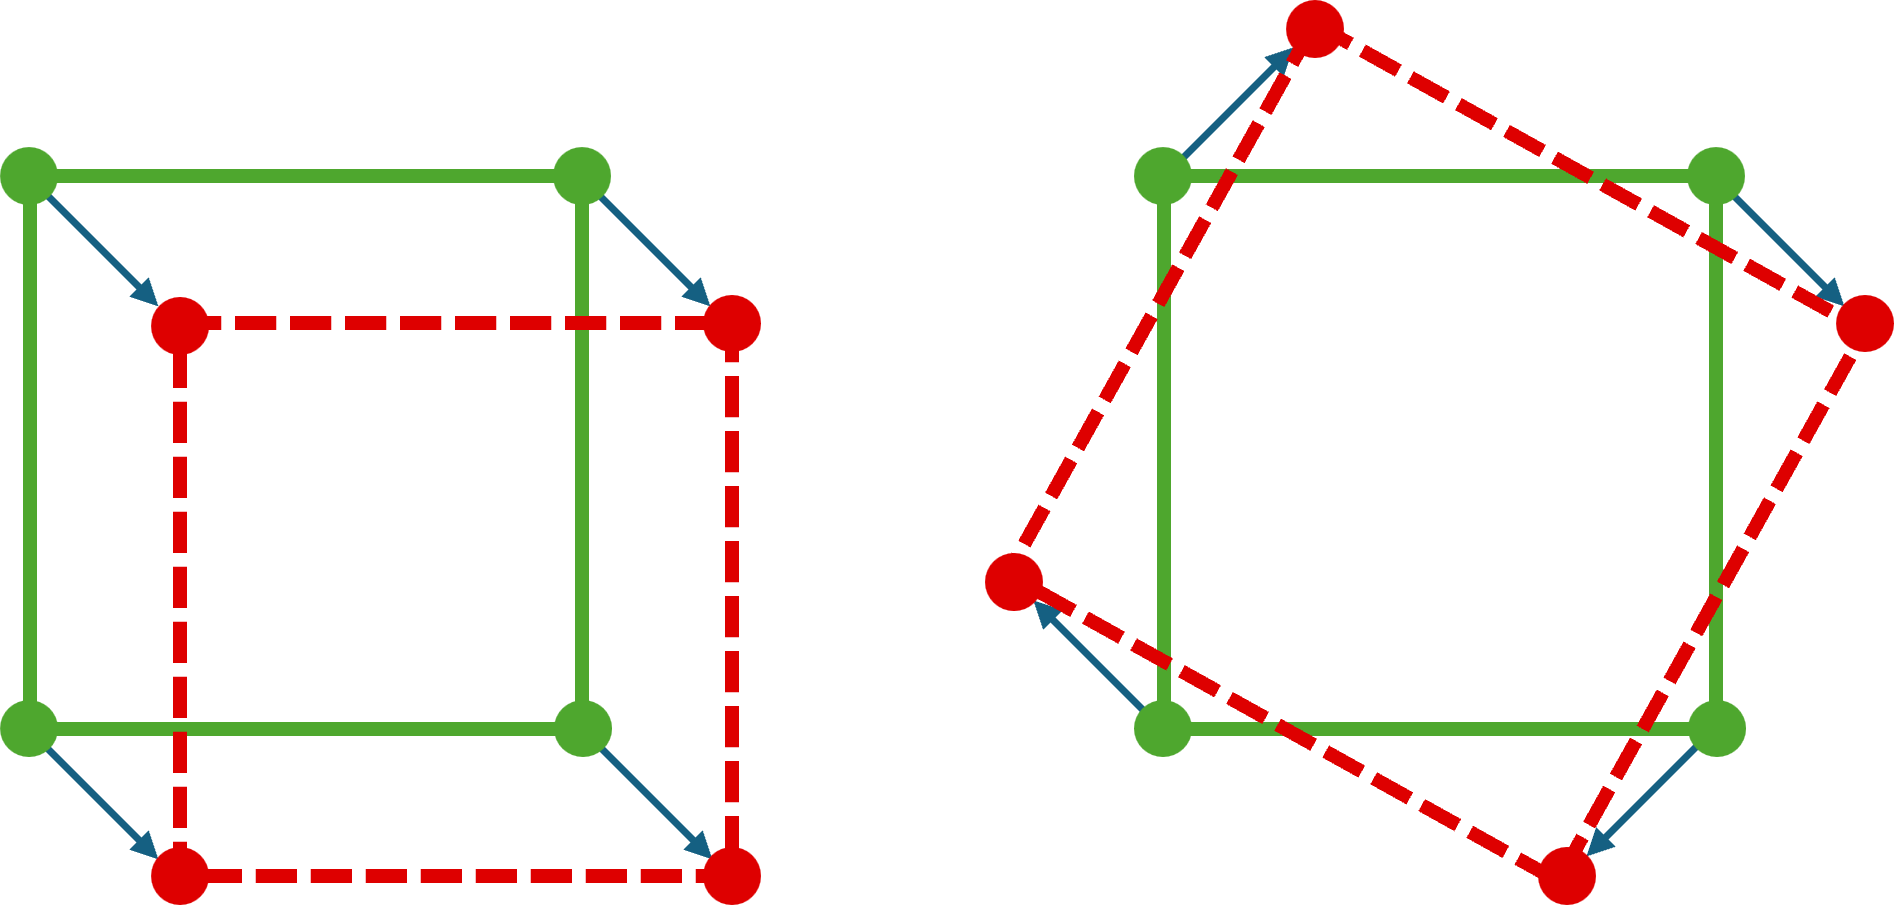
\includegraphics[width=0.7\textwidth]{figures/noise-difference.png}
    \caption{Unlucky noise can affect rotation more than translation}
    \label{fig:noise-difference}
\end{figure}
%TODO maybe we should calculate std dev and show its higher for rotation error (at least i suspect so) since it is more dependent on getting unlucky noise

\subsection{Keypoint noise}
\label{subsec:pixel-noise}
In the second round of tests we change how we apply the random noise to better emulate our system. Since the pixel to world coordinate calculations use the exact view matrix of the camera, the only errors in this part of the algorithm are the result of small floating point inaccuracies. The source of the error will be predominantly a result of the keypoint matching. As such in this second round of tests, we add noise to the pixel coordinates of the keypoints, before converting them to world coordinates. This is more representative of the type of error we will encounter in this system, and so proves a more reliable result. Since the keypoint algorithms used offer sub-pixel precision, we are not limited to only adding integer amounts of pixel noise. As such we use the same random vector method as in the first tests, only this time the vector is 2 dimensional. Since it does not make sense to be adding too small of a fraction of a pixel, as this will have very little effect between runs, we run these tests with a larger granularity of noise magnitude. This does however, allow us to compute the average over 1000 runs, rather than 100, providing more reliable data.\\

\begin{figure}[h]
    \centering
    \begin{subfigure}[t]{0.49\textwidth}
        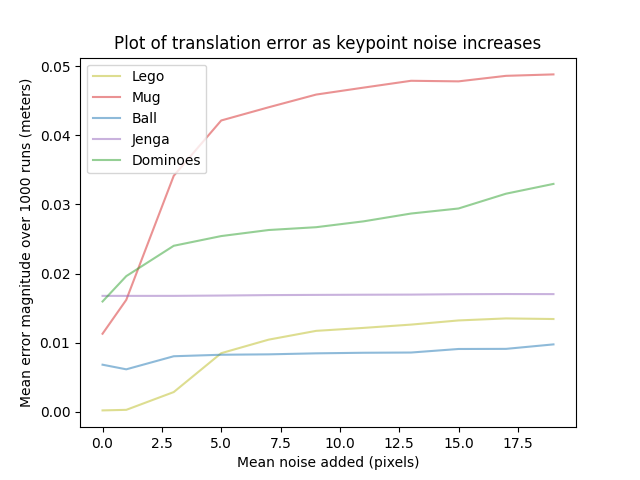
\includegraphics[width=\textwidth]{figures/fig_pixel_noise-translation.png}
        \caption{Noise graph for translation error}
        \label{fig:noise-pixel-translation}
    \end{subfigure}
    \hfill
    \begin{subfigure}[t]{0.49\textwidth}
        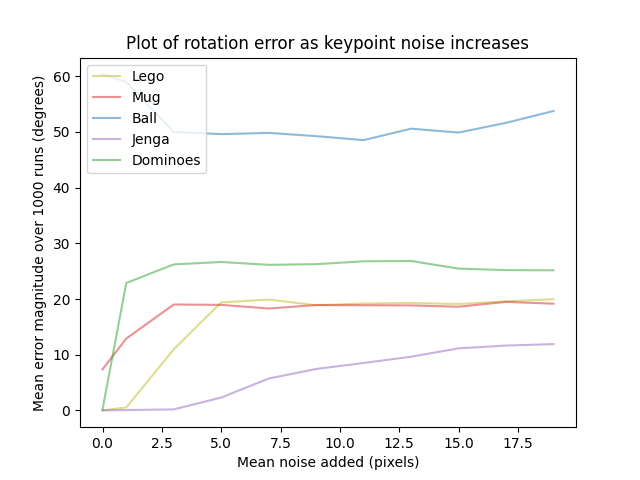
\includegraphics[width=\textwidth]{figures/fig_pixel_noise-rotation.png}
        \caption{Noise graph for rotation error}
        \label{fig:noise-pixel-rotation}
    \end{subfigure}
    \caption{Sensitivity analysis with added keypoint pixel noise}
    \label{fig:noise-pixel}
\end{figure}

\subsubsection{Translation error}
In \reffig{fig:noise-pixel-translation}, objects like the Jenga block and Ball are remarkably stable, with the noise having almost no impact on the computed translation. The Jenga block specifically, exhibits many properties of an ideally marked object for this algorithm. The object has many marked keypoints as discussed earlier. However, it is also one of the largest objects. This means that the noise is proportionally smaller when applied to this object compared to smaller objects like the Lego piece. The object takes up more of the image, and so it takes larger pixel deviations for the noise to have much affect.\\

For the Mug object the error appears to increase more rapidly. This is likely due to the specific topology of this object. The keypoints were marked around the rim of the mug and handle. As such, only small deviations are needed for the keypoint to fall off of or into the mug. In either case, the depth of the keypoint will change wildly. This highlights an important insight. Although the X and Y coordinates of the keypoint can only deviate by as much as the noise maximum, the Z coordinate can change by very large amounts depending on the height of the object. The effect of this is that the error is not uniformly applied to each coordinate. It would be analogous to performing the coordinate noise tests, but with a different much larger magnitude range for the Z coordinate specifically. It is this tendency for small image space deviations to lead to very large world space deviations that accounts for the reduced stability in the pixel noise tests. This is shown in \reffig{fig:unstableZ}.\\

\begin{figure}[h]
    \centering
    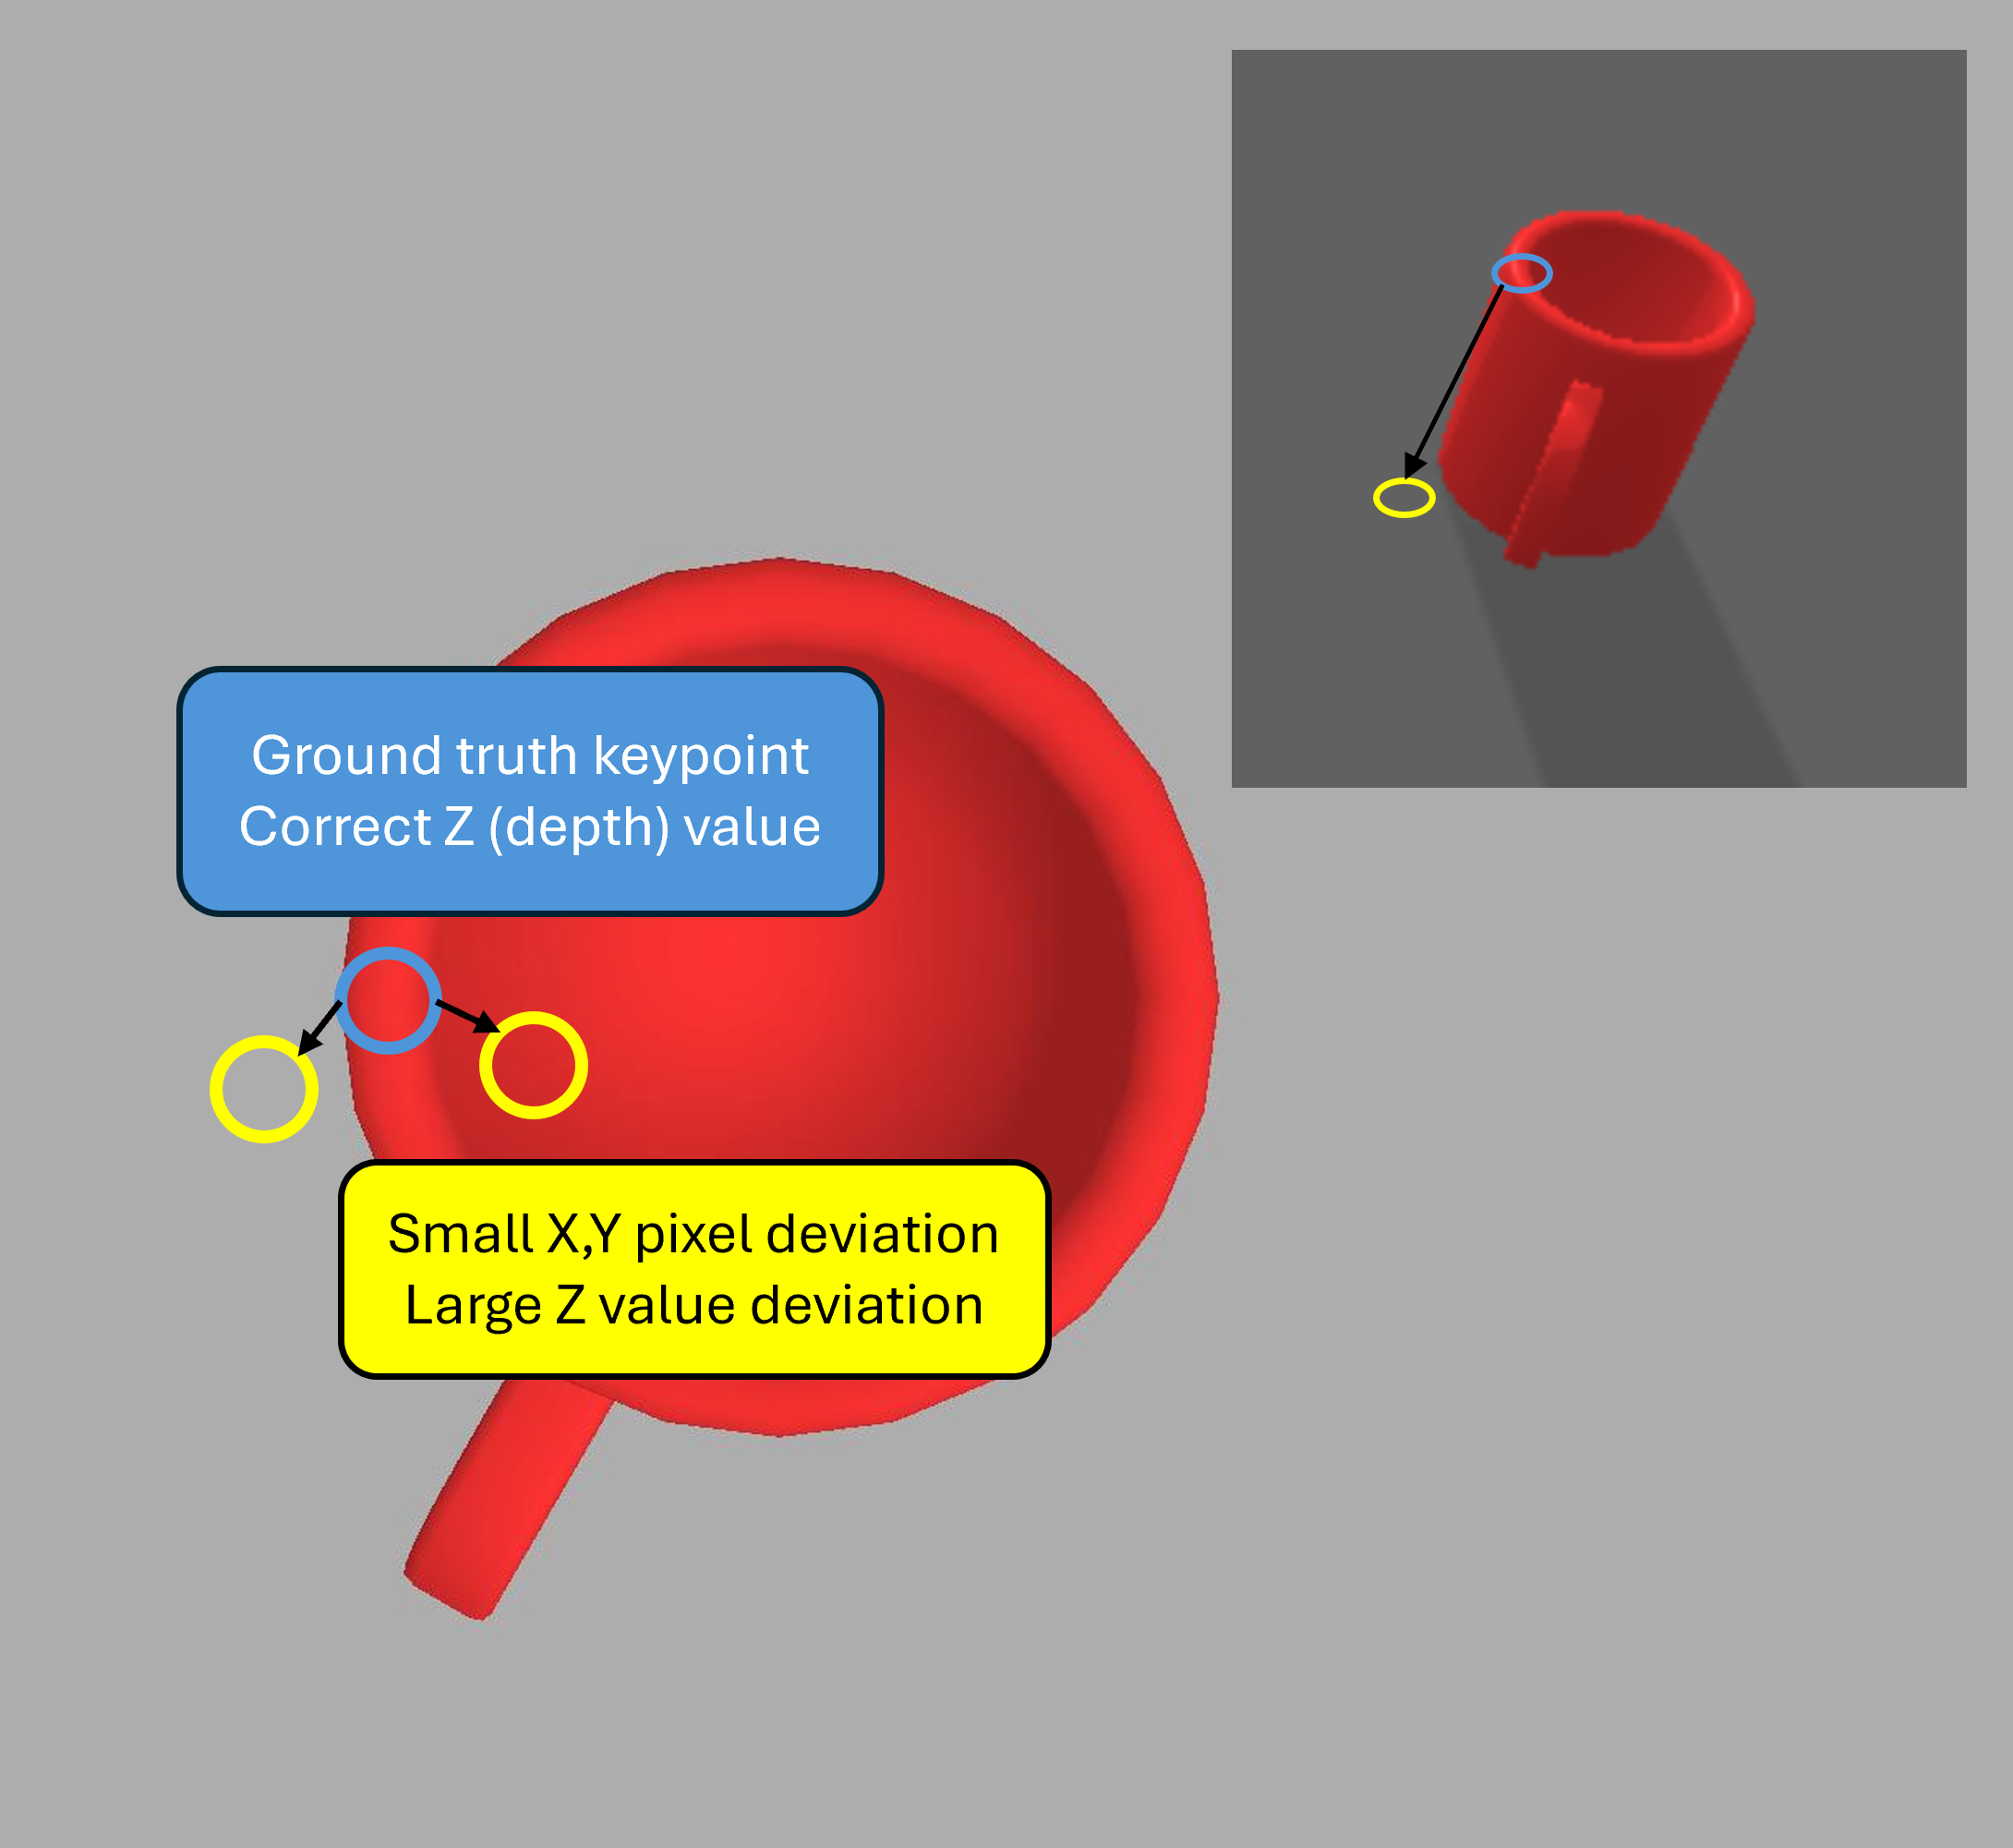
\includegraphics[width=0.5\textwidth]{figures/unstableZ.png}
    \caption{Small X,Y deviations can cause large Z deviations}
    \label{fig:unstableZ}
\end{figure}

To support this theory consider the keypoints marked for the Jenga block object in \refapx{apx:test-suite}. Only 2 of the keypoints are marked on the edge of the object. All other keypoints are in a more central position on the object's face. As such, the deviations of up to even 100 pixels, are not enough to move the majority of these keypoints off of the object and onto the background. As such for this object, the Z coordinate is almost always precisely correct.\\

With regards to how this discovery impacts the true system, it is likely that during normal execution the keypoint matching would not be this poor. The incorrect matches present in the true system are the result of two different keypoints matching to each other. It is unlikely that the system would identify any keypoints which are entirely on the background and not the object. This large Z deviation is a consequence of how the random noise is applied in this test.

\subsubsection{Rotation error}
The rotation error appears to follow similar trends in both the coordinate noise test (\reffig{fig:noise-coord-rotation}) and the pixel noise test (\reffig{fig:noise-pixel-rotation}). For the same reasons as discussed in the previous section, we notice that the rotation error appears less stable than translation, increasing rapidly with small deviations before levelling out. It does not make much difference to the sensitivity of the system, whether the keypoints become rotated from their true position in pixel space or in world space (see \reffig{fig:noise-difference}). The only affect is that the noise applied in pixel space seems to cause smaller deviations overall. This is evident by comparing the two graphs, in both figures the lines follow approximately the same shape, but in \reffig{fig:noise-pixel-rotation} the lines plateau to a lower mean rotation error.\\

Another interesting observation is that the Ball object initially decreases its rotation error as more noise is added. This is certainly unexpected as we would expect noise to make the result worse. This is likely a result of the generally poor rotation calculations for the Ball in general. As discussed in \ref{subsec:coordinate-noise} that by nature of the Ball object being a perfect sphere and the test containing very few marked keypoints, it is very difficult for the system to accurately describe the rotation that occurred. As such we hypothesise that some of the manually marked keypoints were poorly placed, and it happens that adding small amounts of noise can on average move the keypoints closer to where they should have been placed.

\section{Comparison of keypoint algorithms}
\label{sec:algos-test}
In this section we wish to empirically evaluate which keypoint extraction and matching algorithm performs best when used for our system. Any algorithm which can extract and match keypoints could theoretically be used for our system, however this paper focuses analysis on the algorithms discussed in \refsec{sec:keypoint-algos}.\\

We consider two algorithms for keypoint extraction and description, SIFT and ORB. For these rows in the table we apply brute force matching with a suitable distance metric, performing no additional refinement. We add further rows to the table for additional refinement algorithms applied to the initial brute force matches. Despite our outlier filtering originally being designed to be performed after GMS matching, it is possible to apply it immediately to the brute force matches. However, where GMS refines the matches to conform to local smoothness constraints, our method simply removes outliers. Without GMS applied, it is likely that a large number of keypoints will be considered outliers. As such we do not expect this algorithm to perform well, nonetheless it is included to test this hypothesis. The table contains two additional rows, one for applying GMS to the brute force matches, and another for GMS with added outlier filtering.\\

%TODO if we managed more runs then update the number
To conduct the tests we use the same 5 object test suite as with the noise sensitivity tests. For each object we define 5 poses with varying difficulty for the system. We then run LiteBot, using the specified keypoint algorithm to attempt to complete the task on the object in the new pose. Since the whole system is deterministic with respect to the object pose, we do not complete multiple runs with the same object in the same pose. In the table we report the mean translation error, denoted d; the mean rotation error, denoted $\theta$; the mean number of keypoint matches, denoted n; and the success rate of completing the task, denoted s. All averaged across the 5 poses. The results of these tests are presented in \reftab{tab:algo-results}.\\

%TODO populate table
\begin{table}[h!t]
    \begin{adjustbox}{center}
    \setlength{\tabcolsep}{8pt}
    \renewcommand{\arraystretch}{1.05}
    \begin{tabular}{| >{\columncolor{lightgray!25}}c | c | c | c | c | c |}
        \hline
        \rowcolor{lightgray!25}
                    & Lego       & Mug        & Ball       & Jenga      & Domino     \\
        \hline
                    & d=0.0066m  & d=0.0336m  & d=0.0217m  & d=0.0143m  & d=0.0660m  \\
        SIFT        & \er{142.2} & \er{18.6}  & \er{53.3}  & \er{126.3} & \er{137.1} \\
                    & n=9.0      & n=7.0      & n=19.3     & n=42.0     & n=8.0      \\
                    & \s{0}      & \s{0}      & \s{60}     & \s{20}     & \s{0}      \\
        \hline
                    & d=0.0089m  & d=0.0417m  & d=0.0200m  & d=0.0171m  & d=0.0565m  \\
        SIFT        & \er{27.9}  & \er{26.5}  & \er{45.6}  & \er{4.3}   & \er{166.9} \\
        + filtering & n=7.1      & n=5.2      & n=16.4     & n=39.5     & n=5.7      \\
                    & \s{20}     & \s{00}     & \s{60}     & \s{60}     & \s{0}      \\
        \hline
                    & d=0.2350m  & d=0.0569m  & d=0.1210m  & d=0.0162m  & d=0.0583m  \\
        SIFT + GMS  & \er{60.0}  & \er{29.9}  & \er{0.0}   & \er{0.3}   & \er{108}   \\
                    & n=0        & n=1.4      & n=0        & n=19.8     & n=0        \\
                    & \s{0}      & \s{20}     & \s{0}      & \bs{100}   & \s{0}      \\
        \hline
                    & d=0.2350m  & d=0.0569m  & d=0.1210   & d=0.0155m  & d=0.0583m  \\
        SIFT + GMS  & \er{60.0}  & \er{29.9}  & \er{0.0}   & \er{0.3}   & \er{108}   \\
        + filtering & n=0        & n=1.4      & n=0        & n=19.1     & n=0        \\
                    & \s{0}      & \s{20}     & \s{0}      & \bs{100}   & \s{0}      \\ 
        \hline
                    & d=0.0081   & d=0.0112   & d=0.0166   & d=0.0213   & d=0.0341   \\
        ORB         & \er{10.6}  & \er{17.9}  & \er{82.6}  & \er{8.63}  & \er{19.8}  \\
                    & n=204.4    & n=318.0    & n=223.4    & n=2783.8   & n=120.0    \\
                    & \s{80}     & \s{60}     & \bs{80}    & \s{80}     & \s{40}    \\
        \hline
                    & d=0.0067   & d=0.0251   & d=0.0167   & d=0.0194   & d=0.0289   \\
        ORB         & \er{10.9}  & \er{24.7}  & \er{80.6}  & \er{6.40}  & \er{24.9}  \\
        + filtering & n=197.1    & n=247.3    & n=208.7    & n=2605.1   & n=113.6    \\
                    & \s{80}     & \s{40}     & \bs{80}    & \s{80}     & \s{40}    \\
        \hline
                    & d=0.0051   & d=0.0113   & d=0.0207   & d=0.0172   & d=0.0106   \\
        ORB + GMS   & \er{15.8}  & \er{21.2}  & \er{93.3}  & \er{3.57}  & \er{22.5}  \\
                    & n=95.4     & n=113.9    & n=67.0     & n=1531.8   & n=21.0     \\
                    & \s{80}     & \bs{80}    & \bs{80}    & \bs{100}   & \bs{60}   \\
        \hline
                    & d=0.0050   & d=0.0097   & d=0.0207   & d=0.1763   & d=0.0106   \\
        ORB + GMS   & \er{14.7}  & \er{35.6}  & \er{93.3}  & \er{3.49}  & \er{22.5}  \\
        + filtering & n=93.7     & n=80.2     & n=67.0     & n=1289.5   & n=21.0     \\
                    & \bs{100}   & \s{60}     & \bs{80}    & \bs{100}   & \bs{60}    \\
        \hline
    \end{tabular}
    \end{adjustbox}
    \caption{Summary statistics for each algorithm}
    \label{tab:algo-results}  
\end{table}

From these results a number of observations are immediately clear. Most obviously, SIFT keypoints perform much worse than ORB features, across all objects, whichever matching algorithm we use. The key insight is to notice that the average number of matched keypoints is significantly lower than the same setup using ORB. We noticed in \refsec{sec:noise-test}, that the algorithm was more stable when a larger amount of keypoint matches were present. The limited number of keypoints available when using SIFT, contribute to the algorithm's poor performance. Specifically, applying GMS to SIFT features often produce no matches at all. This is because with what few SIFT keypoints we have available, the brute force matching can appear very erratic, with no clear consensus among the matches. As such GMS severely struggles, and can result in a situation with 0 matches. If this is the case, LiteBot is unable to proceed. For this test we consider this an absolute failure. We consider in this case as the system deciding to not move the end effector at all. As a result the end effector error is recorded as the entire offset between the demonstration and live objects. Interestingly, with regards to the rotation error, these cases are not even the highest error achieved by some test runs using SIFT. The largest average error achieved was an angle magnitude of 142.2 degrees. For this test, the robot kept trying to rotate the arm an enormous amount, often hitting into itself and becoming stuck. This large error is a result of the very few keypoints, leading to incredibly unstable calculations when computing the pose offset.\\

With that covered we can turn our attention to the ORB algorithms. The first thing we may notice is that the number of identified keypoint matches is highest when only using ORB and brute force matching. This is to be expected since all the additional matching algorithms refine the existing matches and remove outliers. 
%We may also notice that the outlier filtering removes on average more matches when it is applied directly to ORB matches, than when GMS is also used. This makes sense because 


%TODO put this somewhere
%It is obvious in retrospect that a larger object occupies more pixels of the image. This means that slight deviations in the exact pixels of keypoints have less of an impact on the resulting world coordinates of keypoint matches. It would also provide more possible keypoints to be identified and matched when using the automatic keypoint algorithms. This is something we can control with our demonstrations. By recording demonstrations where the object of interest occupies the majority of the camera frame (by placing the end effector closer to the object when taking the environment context image), the agent will have an easier time computing the correct offset at inference. We also note that the test suite contains 3 demonstrations where the demonstration object is partially out of frame (refer to \refapx{apx:test-suite}). This removes a lot of the potential keypoints of the object, since we already established that edges of the object contain the most keypoint matches. This was a deliberate choice to make the test suite harder, with LiteBot overcoming this issue for the most part as seen in \reftab{tab:algo-results}. Nonetheless, in a practical use case where the user is not trying to actively stress test the system, demonstrations where the object is fully in frame will improve the accuracy of the computed offset.\\

%TODO actually without filtering performed slightly better overall talk about this and justify whichever choice we make
From these tests we conclude that the algorithm which performs best on average is ORB+GMS+filtering. From this evidence we select to implement ORB feature extraction and description, followed by brute force matching, GMS matching and outlier filtering into the final version of LiteBot. We do however note that by removing the outlier filtering step, the performance only decreases slightly. 

Having selected our algorithm, we test a further 5 object poses for each object. We deliberatly choose poses which involve larger offsets between the demonstration and live objects to try to stress test the system. We take average across all objects to calculate the mean success rate of our framework as \textbf{70.0\%}. Since the end effector error and number of matched keypoints depend heavily on the object in question, it would not be appropriate to compute an average for these values. As stated in \refchap{chap:introduction}, we were not able to implement pre-existing One-shot Imitation Learning frameworks, due to their high computational requirements. As a result, we cannot directly compare these algorithms to our own on a consistent test suite. In lieu of this, we compare our results to those produced in the algorithm's original paper.\\

As DINObot influenced many design choices in this framework, it would be pertinent to compare it to our solution. At a high level, the pipeline of our framework and DINObot share many similarities. As such it serves as an excellent base line for our system. The goal of this project was to show that we can take a standard One-shot Imitation Learning system, and exchange the computationally costly AI components with more space efficient classical algorithms, without experiencing a significant loss in performance. In their paper, N. Di Palo and E. Johns demonstrate a task success rate of 80\% on their test suite. While this value is slightly greater than our own, the decrease is marginal. Furthermore, since LiteBot and DINOBot were not tested on the same test suite, it is difficult to draw conclusions about there comparative effectiveness.\\

What we can say for sure is that LiteBot is very capable at completing simple manipulation tasks in our test suite. %TODO

\section{Memory Requirements}
Given that the main motivation for this project was reducing memory requirements, we analyse the amount of RAM a machine would need to run our system. During our previous tests, memory usage peaked at approximately 6.58 GiB across all testing runs. We also emphasise that LiteBot is running entirely on the CPU. No GPU computation time, or VRAM are used. Note, the peak does not represent the total amount of data required by the system. This represents the peak RAM allocated by the system at any one time. Some data, particularly the vision transformer used to initially embed the demonstration and live images, is only needed at the start of the program. After this the memory is freed by garbage collection, and can be re-allocated to later parts of the code. This runtime overhead could be reduced even further by pre-computing embeddings as discussed in \refchap{chap:future}. We perform a rough test to estimate the requirements if we implemented pre-computed embeddings, in which we remove the embedding code from the algorithm and manually tell LiteBot the correct demonstration to use. In this test, the runtime peak RAM usage dropped almost 10 fold to 874 MiB. In a full implementation the embeddings would be loaded from disk and compared, potentially increasing this number slightly. Despite this, it still represents a dramatic runtime decrease. It is however worth noting, that if embeddings are pre-computed this simply moves the problem. When recording and saving demonstrations, the vision transformer would still be required to embed the images once in order to save them to disk, meaning this portion of the framework would still require approximately 6.58GiB. As such the peak memory requirements of the complete system have not changed.\\

Although, it is worth considering that the majority of time spent using the system would be at inference time. The framework is specifically designed to avoid requiring additional demonstrations to be provided later, unless the user wishes to teach additional tasks. As such we can envision a system where a high memory machine can record demonstrations, and distribute these to other low memory machines which only execute the learned algorithm. This could be the case for an industrial application for example, where each individual robot arm of an assembly line does not to be trained independently. Provided they all posses similar robotic hardware, a single robot arm could be trained, and its policy distributed to all arms in a warehouse or factory.\\

Furthermore, the term \socalled{high memory machine} is relative. While 6.58 GiB is obviously more than 0.874 GiB, even this is not particularly high for modern computers. According to the \socalled{Steam Hardware and Software Survey}, conducted in May of 2024 \cite{steam-RAM}, only 2.90\% of Steam users surveyed possessed less than 8GB of RAM. It is important to remember that Steam is a video game store and digital distribution system. As such, all users surveyed will be using their machines for gaming, a use case which often demands high amounts of RAM. While this will skew the results, it remains the most recent survey available at the time of writing. Additionally, Micron \speech{recommend 8GB of RAM for casual computer usage and internet browsing} in 2024 \cite{RAM-req}. Implying that most users, not just those using their system for gaming, should have access to at least 8GB of RAM\footnote{1GB = 1000MB,  1GiB = 1024MiB. It is unclear when the mentioned sources refer to GB if they are actually meaning GiB. However for this comparison, the difference is largely inconsequential.}. From this data we can be reasonably sure that our system would fit within the limitations of the majority of machines in use at this time.\\

In conclusion, the system presented in this paper successfully reduces the minimum memory requirements of a similar One-shot Imitation Learning framework, from some unknown amount greater than 16 GiB, to under 7 GiB. In spite of these reduced memory requirements, LiteBot remains fast, with an average time of 6.11 seconds between taking the live image and aligning to the object, ready to perform the transformed demonstration trajectory. However, this time is dependent on how many demonstrations are learnt and need to be embedded. This would again be reduced, by switching to pre-computed embeddings.



%OLD STUFF
%We will evaluate the success of this project by analysing the proportion of tasks the agent is able to successfully complete. We will compare these results to similar approaches in the field \cite{one-shot-imitation, one-shot-pose-estimate}.
%As described in these papers, the methods used for one-shot imitation learning generalise well to completing the same tasks with different objects. For example picking up a different water bottle to the one in the demonstration. We also know that they generalise to different environment setups, robust to rotations and translations of the objects in the scene. We hope that this project will allow the agent to generalise even further beyond, to skills which differ conceptually to those shown in the demonstrations. We hope that this extra level of generalisability will provide improved success rate metrics on unseen tasks compared to the state of the art current solutions. The existing solutions appear to limit their unseen test set to the same categories of task as their training set, just with new unseen objects. We hope that in this project we can expand this test set to a much more wide spread of potential tasks, and still see high success rates in the testing phase.\\

%In addition to evaluating our algorithm under ideal conditions we would like to investigate how robust it is to its starting configuration. Due to the design of the learning algorithm, it is likely that the ability to learn new skills will be affected by the quality of initial demonstrations. We hypothesise that an agent given 10 unique and diverse demonstrations, will perform better in unseen task completion, than an agent trained with 10 demonstrations which all just involve picking up similar objects. This is because the algorithm as proposed, learns through augmenting existing demonstrations with noise. As such, the skills the agent will learn are likely to conceptually branch off of an existing skill. If the initial skill set is very diverse, then this allows the agent to search a wider portion of the space of all trajectories. Comparatively, if the initial skills are all very similar, then the agent has a harder time searching wide in the search space since it can only save a new skill by augmenting existing skills. A simplified example of this is shown in Figure \ref{fig:trajectory-space} with a 2D search space. In practice the space of all trajectories is far more than 2 dimensions. This makes having diverse initial skills which cover the search space as best as possible even more important since there is far more for the agent to search.

% \begin{figure}[ht]
%     \centering
%     \begin{subfigure}[b]{0.45\textwidth}
%         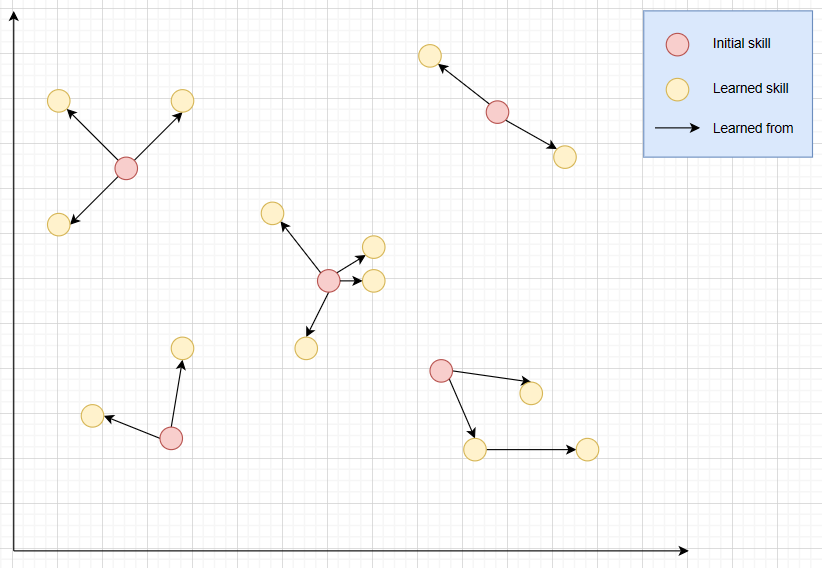
\includegraphics[width=\textwidth]{figures/graph_spread.PNG}
%         \caption{Diverse initial skill set}
%     \end{subfigure}
%     \hfill
%     \begin{subfigure}[b]{0.45\textwidth}
%         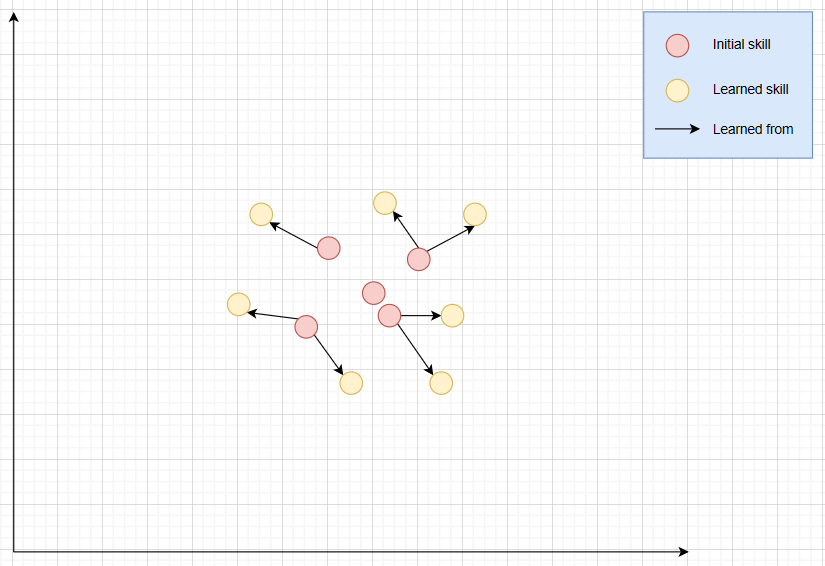
\includegraphics[width=\textwidth]{figures/graph_narrow.PNG}
%         \caption{Narrow initial skill set.}
%     \end{subfigure}
%     \caption{Simplified diagram of trajectory search space.}
%     \label{fig:trajectory-space}
% \end{figure}

% In Figure \ref{fig:trajectory-space} nodes of the graph represent the trajectories which succeed in performing some task and are saved as a skill. Edges represent that the child skill was learned by augmenting the parent skill. Nodes with no parent are the initial skill set, coloured red.